\documentclass[10pt,letterpaper,oneside,openany]{memoir}
\usepackage[margin=0.72in,headheight=16pt,headsep=16pt,footskip=24pt]{geometry}
\usepackage{fontspec,graphicx,xcolor,booktabs,tabularx,array,enumitem,tikz,hyperref}
\usetikzlibrary{arrows.meta,calc,positioning,shapes.geometric}

\setmainfont{Helvetica}
\setsansfont{Helvetica}
\definecolor{reachgold}{HTML}{B87821}
\definecolor{reachvoid}{HTML}{0A1024}
\definecolor{reachblue}{HTML}{477FD4}
\definecolor{reachcopper}{HTML}{CF6D3C}
\definecolor{reachsteel}{HTML}{3D4C5A}
\definecolor{reachmist}{HTML}{E9EDF2}
\definecolor{reachline}{HTML}{AEB8C5}
\hypersetup{colorlinks=true,linkcolor=reachgold,urlcolor=reachblue,pdftitle={The Shattered Reach Rulebook},pdfauthor={Daniel Berger}}

\setsecnumdepth{none}
\setcounter{tocdepth}{1}
\setlength{\parindent}{0pt}
\setlength{\parskip}{5pt plus 1pt}
\setlist{nosep,leftmargin=1.6em}
\renewcommand{\arraystretch}{1.25}

\makepagestyle{reach}
\makeevenhead{reach}{\small\sffamily\color{reachsteel}\textsc{The Shattered Reach}}{}{}
\makeoddhead{reach}{\small\sffamily\color{reachsteel}\textsc{The Shattered Reach}}{}{}
\makeevenfoot{reach}{}{\sffamily\color{reachgold}\thepage}{}
\makeoddfoot{reach}{}{\sffamily\color{reachgold}\thepage}{}
\pagestyle{reach}

\chapterstyle{hangnum}
\renewcommand*{\chapnamefont}{\sffamily\small\color{reachgold}\MakeUppercase}
\renewcommand*{\chapnumfont}{\sffamily\Huge\bfseries\color{reachgold}}
\renewcommand*{\chaptitlefont}{\sffamily\Huge\bfseries\color{reachvoid}}
\setsecheadstyle{\sffamily\Large\bfseries\color{reachsteel}}
\setsubsecheadstyle{\sffamily\large\bfseries\color{reachvoid}}

\newcommand{\game}{\textsc{The Shattered Reach}}
\newcommand{\term}[1]{\textbf{#1}}
\newcommand{\phase}[1]{\textsf{\bfseries\color{reachgold}#1}}
\newcommand{\important}[2]{%
  \par\medskip\noindent
  \colorbox{reachmist}{\parbox{\dimexpr\linewidth-2\fboxsep}{\textsf{\bfseries\color{reachvoid}#1}\quad #2}}
  \par\medskip
}
\newcolumntype{Y}{>{\raggedright\arraybackslash}X}
\makeatletter
\newcommand{\inlinecontents}{%
  \par\bigskip
  {\sffamily\Large\bfseries\color{reachsteel}Contents\par}\smallskip
  \@starttoc{toc}%
}
\makeatother

\begin{document}
\begin{titlingpage}
\begin{tikzpicture}[remember picture,overlay]
  \fill[reachvoid] (current page.south west) rectangle (current page.north east);
  \shade[inner color=reachblue!35,outer color=reachvoid] ($(current page.south west)+(2.3in,4.7in)$) circle (2.6in);
  \shade[inner color=reachcopper!26,outer color=reachvoid] ($(current page.south east)+(-2.1in,4.1in)$) circle (2.4in);
  \foreach \x/\y/\r in {.8/1.0/.7,1.2/6.7/.8,1.8/9.3/.55,2.2/3.5/.65,2.9/7.1/.5,3.4/1.5/.7,3.8/5.7/.45,4.4/8.2/.8,4.9/2.6/.55,5.5/6.3/.65,6.1/9.6/.5,6.7/1.1/.7,7.0/5.4/.5,7.7/8.0/.8}
    \fill[white,opacity=.62] ($(current page.south west)+(\x in,\y in)$) circle (\r pt);
  \draw[reachgold,line width=1.2pt] ($(current page.north west)+(0.72in,-0.65in)$) -- ($(current page.north east)+(-0.72in,-0.65in)$);
  \draw[reachgold,line width=1.2pt] ($(current page.south west)+(0.72in,0.65in)$) -- ($(current page.south east)+(-0.72in,0.65in)$);

  \node[anchor=north,align=center,text=white] at ($(current page.north)+(0,-0.95in)$) {%
    \sffamily\bfseries\fontsize{18}{20}\selectfont\color{reachgold} THE\\[-1pt]
    \fontsize{40}{42}\selectfont\color{white} SHATTERED\\[-3pt]
    \fontsize{40}{42}\selectfont\color{reachgold} REACH};

  \node[rotate=-62] at ($(current page.south west)+(2.35in,4.55in)$) {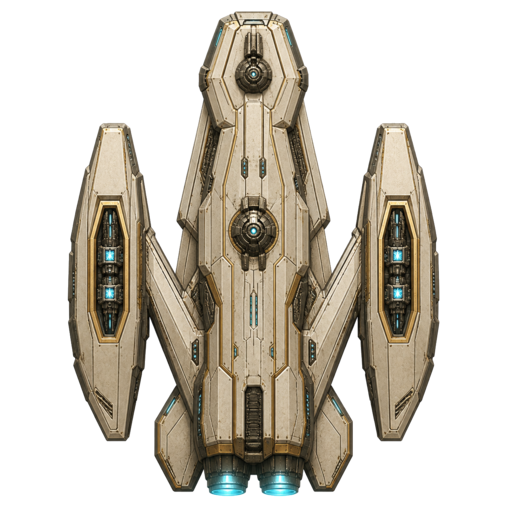
\includegraphics[width=2.75in]{../../app/assets/images/ships/tactical/aurelian_cruiser.png}};
  \node[rotate=62] at ($(current page.south west)+(6.2in,4.45in)$) {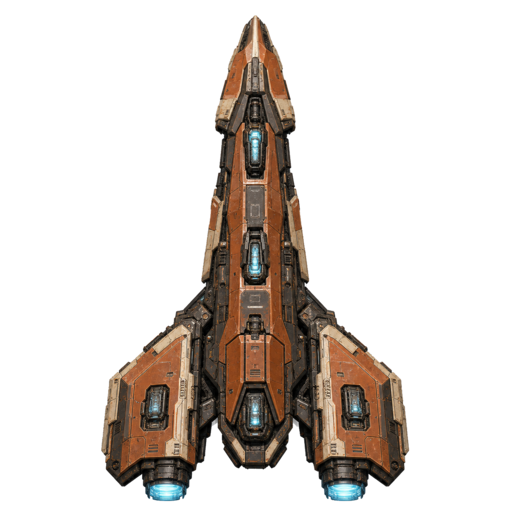
\includegraphics[width=2.55in]{../../app/assets/images/ships/tactical/kestrel_cruiser.png}};

  \draw[reachblue!45,line width=8pt,opacity=.22] ($(current page.south west)+(3.22in,4.95in)$) -- ($(current page.south west)+(5.16in,4.70in)$);
  \draw[white,line width=3.2pt,opacity=.9] ($(current page.south west)+(3.22in,4.95in)$) -- ($(current page.south west)+(5.16in,4.70in)$);
  \draw[cyan!70,line width=1.4pt] ($(current page.south west)+(3.22in,4.95in)$) -- ($(current page.south west)+(5.16in,4.70in)$);
  \draw[reachgold,line width=2.2pt,dash pattern=on 3pt off 5pt] ($(current page.south west)+(5.42in,4.18in)$) -- ($(current page.south west)+(3.52in,4.02in)$);
  \fill[white] ($(current page.south west)+(5.16in,4.70in)$) circle (3.2pt);
  \foreach \a in {0,30,...,330} {\draw[reachcopper,line width=1.2pt] ($(current page.south west)+(5.16in,4.70in)$) -- ++(\a:.18in);}

  \node[anchor=south,align=center,text=white,text width=6.5in] at ($(current page.south)+(0,1.35in)$) {\sffamily\Large A tactical game of secret power, impulse movement, and fleet command};
  \node[anchor=south,text=white!68] at ($(current page.south)+(0,.82in)$) {\sffamily\small Complete prototype rulebook \textbullet\ Version 0.2};
\end{tikzpicture}
\null
\end{titlingpage}

\frontmatter
\phantomsection
\addcontentsline{toc}{chapter}{The Shattered Reach}
{\sffamily\Huge\bfseries\color{reachvoid}The Shattered Reach\par}\medskip

For two centuries, the \term{Meridian Gates} bound the Reach into a single civilization. Named for the celestial reference lines by which navigators fixed their position, the gates established equally dependable meridians across interstellar space. Worlds measured distance by minutes rather than light-years.

Then every gate fired at once. Worlds vanished behind walls of distorted space, fleets were cut in half, and the star maps became lies. The survivors remember that night simply as the \term{Shattering}.

Eighty-seven years later, the dead lanes flicker back to life, opening brief corridors to abandoned arsenals, isolated colonies, and systems unseen for generations. Whoever holds the anchor stations can decide which worlds reconnect---and on whose terms.

The \term{Aurelian Compact} claims a duty to restore the old union. The \term{Veyr Dominion} means to replace it with an order strong enough to survive the next collapse. The \term{Kestrel Freeholds} fight to keep the frontier unowned. Their wars are small by necessity: a handful of ships, minutes before a corridor closes, and entire systems in the balance.

\important{YOUR BATTLE}{Each engagement represents one of these brief, decisive contests: rival commands enter a newly opened lane, fight for control, and try to escape before the route becomes unstable again.}

\inlinecontents
\clearpage
\mainmatter
\chapter{Overview and Setup}

In \game{}, two commanders guide small fleets across a hex map. Every turn, commanders secretly divide reactor output among movement, direct-fire weapons, shield reinforcement, and repairs. A semi-random impulse deck determines when each speed moves. After movement, missiles launch and direct-fire weapons engage.

\section{Ships and ship displays}

Every ship has four kinds of systems:

\begin{description}[style=nextline,leftmargin=0pt]
  \item[Reactor / engines] Each undamaged engine box provides one energy each turn. Engine damage reduces future available energy.
  \item[Hull integrity] Hull boxes measure the ship's survival. When every hull box is damaged, the ship is immediately destroyed.
  \item[Forward and aft shields] Shields absorb incoming damage before internal systems are hit. Their current strength is public information.
  \item[Weapons] The engineering silhouette shows each weapon's physical mount, firing arc, energy cost, damage boxes, and missile ammunition where applicable.
\end{description}

Use blue markers for available and allocated energy, yellow markers for intact shield boxes, and red markers for damage when playing on the tabletop. The browser version records these automatically.

\section{Weapons at a glance}

\begin{description}[style=nextline,leftmargin=0pt]
  \item[Lance beams] Accurate and destructive, but short-ranged and expensive to charge.
  \item[Mass drivers] Less accurate, but inexpensive to charge and effective at longer range.
  \item[Seeker missiles] Require no energy and have unlimited pursuit range, but launchers carry limited ammunition. Missile counters move independently on the map.
\end{description}

\section{Choose a battle}

Each commander selects one to three ships. Ship types may be repeated. For a roughly balanced battle, either use the same number and classes of ships or compare size values:

\begin{center}
\begin{tabular}{lccc}\toprule
Hull class & Small & Medium & Large\\\midrule
Size value & 2 & 3 & 4\\\bottomrule
\end{tabular}
\end{center}

The Command AI can match the player's fleet by ship count or by total size value. The original duel format uses one or two ships per side, usually of equal class.

\section{Prepare the battlefield}

\begin{enumerate}
  \item Choose a flat-top hex map measuring 12 by 12, 15 by 15, or 20 by 20 hexes. A tabletop map should not exceed 20 by 20.
  \item Place opposing fleets \term{10 to 15 hexes apart}, generally facing one another. Spread multiple ships into nearby unoccupied hexes.
  \item Fill every forward shield, aft shield, hull, and reactor box shown on each ship display.
  \item Give every small and medium ship one special-maneuver token. Large ships do not receive one.
  \item Place the listed ammunition beside each missile launcher. Unless a ship sheet says otherwise, a launcher begins with three missiles.
  \item Separate the twelve impulse cards into their three phase decks of four cards each. Shuffle each deck independently.
  \item If using optional rules, agree on them before beginning allocation.
\end{enumerate}

\important{PUBLIC AND SECRET INFORMATION}{Ship position, facing, speed after announcement, damage, remaining shields, expended missiles, and used special maneuvers are public. Energy allocation remains secret until both sides commit it.}

\chapter{Turn Sequence and Energy}

Each turn has an allocation segment followed by twelve impulses. Each impulse contains movement, missile launch, and direct-fire steps in that order.

\section{Complete sequence of play}

\begin{enumerate}
  \item \phase{Allocate Energy.} Each commander secretly plans every surviving ship.
  \item \phase{Commit Fleets.} When both commands are ready, reveal allocations and announce each ship's speed.
  \item \phase{Determine Initiative.} Each side rolls one die; the high roll wins. Re-roll ties.
  \item \phase{Resolve Twelve Impulses.}
  \begin{enumerate}[label=\alph*.]
    \item Draw the next card from the current phase deck.
    \item Move every ship whose speed appears, slowest first. Then move all missiles already on the map.
    \item Launch any missiles.
    \item Fire any eligible lance beams and mass drivers.
  \end{enumerate}
  \item \phase{Check Victory.} Resolve destruction and determine whether the battle has ended.
  \item \phase{End the Turn.} Complete funded shield repairs, clear expended allocations, reset unfired status, and begin a new turn.
\end{enumerate}

\section{Allocate energy}

Each undamaged reactor / engine box generates one energy. Secretly assign that energy among:

\begin{itemize}
  \item \term{Speed}: one energy buys one point of speed, from 0 to 12.
  \item \term{Lance beams}: two energy charges one beam weapon.
  \item \term{Mass drivers}: one energy charges one mass-driver weapon.
  \item \term{Shield reinforcement}: one energy absorbs one damage against the chosen shield during this turn.
  \item \term{Shield repair}: two energy schedules one damaged shield box for restoration at the end of the turn.
  \item \term{Weapon repair}: three energy repairs one eligible direct-fire weapon when that optional rule is enabled.
\end{itemize}

Missiles require no energy. A commander is never required to spend all available energy; unspent energy is lost when the allocation is committed.

When commanding multiple ships, complete and save a plan for each surviving ship before committing the fleet. Committing makes every ship's plan final for the turn.

\section{Announce speed and initiative}

After both commands commit, announce every ship's speed. All other allocation details also become public in tabletop play. Each side rolls one die for initiative; high roll wins, with ties re-rolled.

Initiative settles simultaneous choices. When equal-speed ships are due to move, the side with initiative determines the order. If both sides want to use a special maneuver at the same moment, initiative decides which resolves first. It likewise settles ambiguous shield facings and, where necessary, firing declarations.

\section{Impulse decks}

The twelve cards are arranged as three separately shuffled phase decks:

\begin{center}
\begin{tabular}{lccc}\toprule
Impulses & 1--4 & 5--8 & 9--12\\\midrule
Deck & Phase 1 & Phase 2 & Phase 3\\\bottomrule
\end{tabular}
\end{center}

Each card lists the speeds that receive one movement opportunity. A ship moves if its announced speed appears on the card. Across the complete twelve-card sequence, a ship moving at speed $N$ receives exactly $N$ movement opportunities.

\important{SLOWEST FIRST}{Resolve eligible ships from lowest speed to highest speed. When two ships have the same speed, use initiative to determine their order. Every eligible ship receives its own movement choice.}

\section{Worked impulse}

Suppose an impulse card lists speeds 4, 6, 8, 10, and 12. A speed-4 enemy cruiser and two friendly speed-6 frigates are on the map.

\begin{enumerate}
  \item The speed-4 cruiser resolves its movement first.
  \item The two speed-6 frigates then resolve separately in the order determined by initiative. One may move forward while the other side-slips.
  \item All missiles launched in earlier impulses move up to two hexes toward their assigned targets.
  \item Ships may launch new missiles. Those missiles remain in their launch hex during this impulse.
  \item Eligible ships may fire charged lance beams and mass drivers, one weapon at a time.
  \item When both sides finish firing, end the impulse and draw the next card.
\end{enumerate}

\chapter{Movement}

Ships and missiles move only during the movement step of an impulse. Ships move forward relative to their facing; they never move backward.

\section{Ship movement choices}

When a ship's speed appears on the impulse card, choose one legal action:

\begin{itemize}
  \item move forward one hex without changing facing;
  \item side-slip one forward-diagonal hex without changing facing;
  \item turn 60 degrees in place after satisfying turn mode; or
  \item lose the movement if no legal maneuver exists.
\end{itemize}

\begin{center}
\begin{tikzpicture}[
  scale=.78,
  >=Latex
]
  % Flat-top hexes meet across their edges. Their neighboring centers lie at
  % 30, 90, 150, 210, 270, and 330 degrees---not at the vertices.
  \coordinate (forward) at (0,1.022in);
  \coordinate (port) at (-.885in,.511in);
  \coordinate (starboard) at (.885in,.511in);
  \coordinate (west) at (-.885in,-.511in);
  \coordinate (aft) at (0,-1.022in);
  \coordinate (east) at (.885in,-.511in);

  % Draw exact .59-inch-radius hexes so neighboring cells share an edge
  % without the hidden padding introduced by TikZ polygon nodes.
  \foreach \cell in {west,aft,east} {
    \begin{scope}[shift={(\cell)}]
      \draw[reachline]
        (.59in,0) -- (.295in,.511in) -- (-.295in,.511in) --
        (-.59in,0) -- (-.295in,-.511in) -- (.295in,-.511in) -- cycle;
    \end{scope}
  }
  \begin{scope}[shift={(forward)}]
    \draw[reachgold,fill=reachgold!10]
      (.59in,0) -- (.295in,.511in) -- (-.295in,.511in) --
      (-.59in,0) -- (-.295in,-.511in) -- (.295in,-.511in) -- cycle;
  \end{scope}
  \foreach \cell in {port,starboard} {
    \begin{scope}[shift={(\cell)}]
      \draw[reachblue,fill=reachblue!8]
        (.59in,0) -- (.295in,.511in) -- (-.295in,.511in) --
        (-.59in,0) -- (-.295in,-.511in) -- (.295in,-.511in) -- cycle;
    \end{scope}
  }
  \draw[reachgold,line width=1.2pt,fill=reachgold!5]
    (.59in,0) -- (.295in,.511in) -- (-.295in,.511in) --
    (-.59in,0) -- (-.295in,-.511in) -- (.295in,-.511in) -- cycle;

  \draw[->,line width=2pt,reachgold] (0,.18in) -- ($(forward)+(0,-.18in)$);
  \draw[->,densely dashed,line width=1.6pt,reachblue] (-.13in,.08in) -- ($(port)+(.16in,-.09in)$);
  \draw[->,densely dashed,line width=1.6pt,reachblue] (.13in,.08in) -- ($(starboard)+(-.16in,-.09in)$);

  \node[font=\sffamily\small\bfseries,text=reachgold,align=center] at ($(forward)+(0,.18in)$) {FORWARD};
  \node[font=\sffamily\scriptsize\bfseries,text=reachblue,align=center,text width=.82in]
    at ($(port)+(0,.19in)$) {PORT\\SLIP};
  \node[font=\sffamily\scriptsize\bfseries,text=reachblue,align=center,text width=.82in]
    at ($(starboard)+(0,.19in)$) {STARBOARD\\SLIP};

  % The side-slip destinations retain the ship's original north-facing heading.
  % The forward movement arrow already communicates that heading on its own.
  \foreach \cell in {port,starboard} {
    \draw[->,line width=.9pt,reachsteel]
      ($(\cell)+(0,-.34in)$) -- ($(\cell)+(0,-.17in)$);
  }

  \node[inner sep=0pt] at (0,.03in) {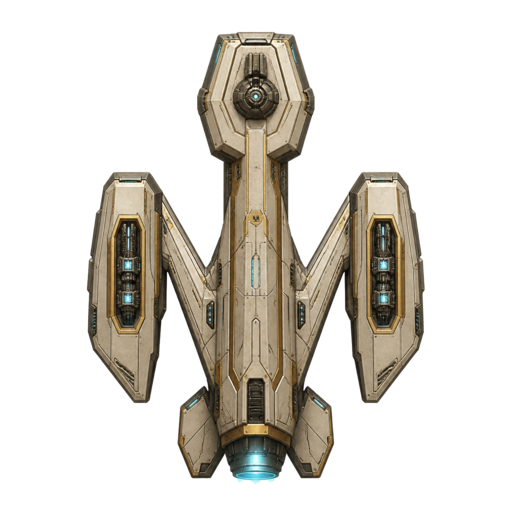
\includegraphics[width=.64in]{../../app/assets/images/ships/tactical/aurelian_frigate.png}};
  \draw[->,line width=1.3pt,reachcopper]
    ($(0,.08in)+(90:.35in)$) arc[start angle=90,end angle=150,radius=.35in];
  \draw[->,line width=1.3pt,reachcopper]
    ($(0,.08in)+(90:.35in)$) arc[start angle=90,end angle=30,radius=.35in];
  \node[font=\sffamily\scriptsize\bfseries,text=reachcopper,align=center]
    at (0,-.42in) {TURN 60\textdegree};
  \node[font=\sffamily\scriptsize,text=reachblue,align=center] at (0,-1.78in)
    {DASHED ARROW: move to another hex; keep facing north};
  \node[font=\sffamily\scriptsize,text=reachcopper,align=center] at (0,-1.98in)
    {CURVED ARROW: remain in the hex; rotate 60\textdegree};
\end{tikzpicture}
\end{center}

\section{Turn mode}

A ship's \term{turn mode} is the number of hexes it must translate forward before it may turn again. Moving forward and side-slipping both add one to this count. Turning resets the count to zero.

\begin{center}
\begin{tabular}{lccc}\toprule
Hull class & Speed 1--4 & Speed 5--8 & Speed 9--12\\\midrule
Small & 0 & 1 & 2\\
Medium & 1 & 2 & 3\\
Large & 2 & 3 & 4\\\bottomrule
\end{tabular}
\end{center}

A speed-0 ship does not receive a normal movement opportunity. A turn mode of 0 permits a ship to turn on every movement opportunity, including repeatedly turning in place under the standard rules.

\section{Side-slipping}

A side-slip moves the ship into either forward-diagonal hex while preserving its facing. It represents a more granular course change than the hex grid otherwise permits.

A ship may not side-slip twice in succession. It must move forward or turn before it may side-slip again. A side-slip counts as forward movement for satisfying turn mode.

\section{Occupied hexes and the map edge}

A ship may never enter a hex occupied by another ship. It must choose another legal movement or turn if possible, using its special maneuver if necessary and available. If no legal choice exists, the movement is lost.

Missiles may share hexes with ships and other missiles. A missile that enters its assigned target's hex immediately impacts.

A ship that leaves the map for any reason is destroyed for all purposes, including victory scoring.

\section{Missile movement}

Missiles move at speed 24: two one-hex moves during the movement step of every impulse. They have turn mode 0 and must use each move to approach their assigned target. If a missile reaches the target after its first hex of movement, it impacts immediately and does not take a second move.

Missiles launch \emph{after} movement. A newly launched missile is placed in its launching ship's hex and does not move during that impulse. It begins moving in the following impulse. If its target is destroyed before impact, the missile loses lock and is removed.

\section{Special maneuvers}

Every small and medium ship begins the game with one special-maneuver token. Large ships do not. The token may be spent once per game during that ship's movement opportunity, either immediately before or immediately after its normal movement.

\begin{description}[style=nextline,leftmargin=0pt]
  \item[Bootlegger] Rotate the ship to any facing, ignoring normal turn-mode restrictions. This counts as a turn and resets forward hexes accumulated toward the next turn.
  \item[Quick Stop] Set the ship's speed to 0. It receives no more normal movement opportunities that turn.
  \item[Emergency Power] Immediately move one extra hex straight forward. The destination must be open.
\end{description}

Once spent, the token is unavailable for the rest of the battle.

\chapter{Combat}

Combat follows movement in every impulse. Resolve missile launches before any lance beam or mass driver fires.

\section{Missile launch step}

Any undestroyed, unfired missile launcher with ammunition may launch one seeker missile. Launching costs no energy. Choose an enemy ship as the target, reduce that launcher's ammunition by one, mark the launcher fired for the turn, and place a missile counter in the launcher's hex.

Missiles have a 360-degree launch arc and unlimited pursuit range. They may target ships, never other missiles. Each missile retains its declared target until impact or until that target is destroyed.

If a missile launcher is destroyed, all ammunition remaining in that launcher is lost. This causes no secondary explosion.

\section{Direct-fire step}

After both sides finish launching missiles, eligible ships may fire lance beams and mass drivers. A direct-fire weapon may fire when all of the following are true:

\begin{itemize}
  \item it was charged during this turn's energy allocation;
  \item it has not already fired this turn;
  \item it has not been destroyed or repaired during this turn;
  \item the target is within the weapon's maximum range; and
  \item the target lies within at least one of the weapon's listed firing arcs.
\end{itemize}

Select one weapon, then one legal enemy ship or hostile missile. Determine range, identify the range band, and roll one die. A result equal to or greater than the listed hit number scores a hit. Mark the weapon fired and remove its allocated energy even if it misses.

Count range by including the target's hex and excluding the firing ship's hex.

\section{Weapon matrix}

\begin{center}
\small
\begin{tabularx}{\linewidth}{l c Y Y Y}\toprule
Weapon & Energy & Short & Medium & Long\\\midrule
Lance beam & 2 & 1--3; 2+; 3 damage & 4--6; 3+; 2 damage & 7--9; 4+; 1 damage\\
Mass driver & 1 & 1--4; 3+; 2 damage & 5--8; 4+; 2 damage & 9--12; 5+; 2 damage\\
Seeker missile & 0 & \multicolumn{3}{l}{Unlimited pursuit range; automatic impact for 3 damage.}\\\bottomrule
\end{tabularx}
\end{center}

\section{Firing at missiles}

Lance beams and mass drivers may target hostile missiles, including missiles launched during the current impulse. Apply a $-1$ penalty to the attack die roll; equivalently, increase the required hit number by one. A successful hit at any range destroys the missile. Damage values do not matter against missiles.

\section{Firing arcs}

Each direct-fire weapon lists one or more arcs:

\begin{description}[style=nextline,leftmargin=0pt]
  \item[F --- Forward] The three directions centered on the ship's bow.
  \item[L --- Port] The three directions extending from the ship's left side.
  \item[R --- Starboard] The three directions extending from the ship's right side.
  \item[A --- Aft] The three directions centered on the ship's stern.
\end{description}

Each arc begins in the three adjacent hexes and extends outward indefinitely. Arcs overlap: the forward-port direction lies in both the Forward and Port arcs, for example. A weapon may fire if the target lies in any listed arc. A 360-degree weapon can engage in every direction.

\begin{center}
\begin{tikzpicture}[scale=.76]
  \coordinate (forward) at (0,1.022in);
  \coordinate (forwardport) at (-.885in,.511in);
  \coordinate (forwardstarboard) at (.885in,.511in);
  \coordinate (aftport) at (-.885in,-.511in);
  \coordinate (aft) at (0,-1.022in);
  \coordinate (aftstarboard) at (.885in,-.511in);
  \colorlet{forwardportarc}{reachgold!50!reachblue}
  \colorlet{forwardstarboardarc}{reachgold!50!reachsteel}
  \colorlet{aftportarc}{reachblue!50!reachcopper}
  \colorlet{aftstarboardarc}{reachsteel!50!reachcopper}

  % Use the same exact flat-top geometry as the tactical map. Mixed colors on
  % the diagonal hexes reinforce that boundary directions belong to two arcs.
  \foreach \cell/\arcfill in {
    forward/reachgold,
    forwardport/forwardportarc,
    forwardstarboard/forwardstarboardarc,
    aftport/aftportarc,
    aft/reachcopper,
    aftstarboard/aftstarboardarc} {
    \begin{scope}[shift={(\cell)}]
      \draw[draw=\arcfill,line width=1pt,fill=\arcfill!18]
        (.59in,0) -- (.295in,.511in) -- (-.295in,.511in) --
        (-.59in,0) -- (-.295in,-.511in) -- (.295in,-.511in) -- cycle;
    \end{scope}
  }

  \node[font=\sffamily\large\bfseries,text=reachvoid] at (forward) {F};
  \node[font=\sffamily\large\bfseries,text=reachvoid] at (forwardport) {F/L};
  \node[font=\sffamily\large\bfseries,text=reachvoid] at (forwardstarboard) {F/R};
  \node[font=\sffamily\large\bfseries,text=reachvoid] at (aftport) {A/L};
  \node[font=\sffamily\large\bfseries,text=reachvoid] at (aft) {A};
  \node[font=\sffamily\large\bfseries,text=reachvoid] at (aftstarboard) {A/R};

  \draw[reachgold,line width=1.4pt,fill=reachvoid]
    (.59in,0) -- (.295in,.511in) -- (-.295in,.511in) --
    (-.59in,0) -- (-.295in,-.511in) -- (.295in,-.511in) -- cycle;
  \node[inner sep=0pt] at (0,0) {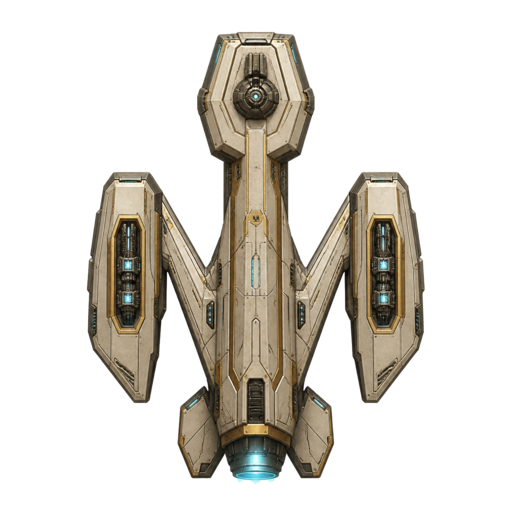
\includegraphics[width=.66in]{../../app/assets/images/ships/tactical/aurelian_frigate.png}};
  \draw[->,reachgold,line width=1.2pt] (0,.30in)--(0,.72in);

  \node[align=center] at (0,-1.78in) {Adjacent arc reference; the frigate's bow points north.\\Each labeled direction continues outward from the ship.};
\end{tikzpicture}
\end{center}

\important{FIRE ONCE}{Each weapon mount may fire only once per turn. Multiple identical mounts shown on a ship are separate weapons and may be fired independently.}

\chapter{Shields, Damage, and Repair}

\section{Shield facing}

Every ship has a forward shield and an aft shield. An attack arriving through the forward half of the ship strikes the forward shield; an attack through the rear half strikes the aft shield. If the line of fire lies exactly on the boundary, the side with initiative chooses which bank is hit.

Shields are always active while at least one box remains; they do not require energy merely to function.

\section{Shield reinforcement}

During allocation, assign reinforcement separately to the forward and aft banks. Each reinforcement energy absorbs one damage against that bank during the current turn. Reinforcement is lost when used and does not restore permanent shield boxes.

The reinforcement limit applies independently to each shield bank:

\begin{center}
\begin{tabular}{lccc}\toprule
Hull class & Small & Medium & Large\\\midrule
Maximum reinforcement per bank & 1 & 2 & 3\\\bottomrule
\end{tabular}
\end{center}

A completely collapsed shield cannot be reinforced. It may still be repaired.

\section{Resolve a hit}

Apply each hit in this order:

\begin{enumerate}
  \item Determine whether the forward or aft shield was struck.
  \item Remove reinforcement assigned to that bank, one point per damage.
  \item Remove permanent shield boxes from that bank, one per remaining damage.
  \item For every point still remaining, roll once on the Internal Damage table.
\end{enumerate}

\begin{center}
\begin{tabularx}{.82\linewidth}{c l Y}\toprule
Die & Result & Effect\\\midrule
1--3 & Hull & Damage one hull box. Destroy the ship immediately when no hull boxes remain.\\
4--5 & Engine & Damage one reactor / engine box. The ship generates one less energy on later turns.\\
6 & Weapon & The owning player chooses one undestroyed weapon and marks it destroyed. If none remain, apply one hull damage instead.\\\bottomrule
\end{tabularx}
\end{center}

A weapon is destroyed by one damage even if its energy cost is represented by multiple boxes. Destroying a missile launcher also destroys all ammunition still assigned to that launcher.

\section{Shield repair}

If either shield is below its printed maximum, spend two energy during allocation and choose the forward or aft bank. At the end of the turn, restore one box to that bank. A ship may repair a completely collapsed shield. Only one shield box may be repaired by a ship per turn.

\section{Optional weapon repair}

When the Weapon Repair option is enabled, spend three energy during allocation to repair one destroyed lance beam or mass driver. Missile launchers cannot be repaired. The repaired weapon is restored when allocation is committed but remains offline for that entire turn; it may be charged normally on the following turn.

\section{End of turn}

After the twelfth impulse:

\begin{enumerate}
  \item check victory conditions;
  \item complete each funded shield repair;
  \item return energy to every undamaged reactor / engine box;
  \item discard unused shield reinforcement and all other allocations;
  \item ready surviving weapons that were fired, except weapons repaired during the ending turn;
  \item reset turn-mode progress and begin secret allocation for the next turn.
\end{enumerate}

Destroyed engine boxes generate no energy.

\section{Victory points and victory}

For a scored tabletop battle, gain one victory point for every enemy hull box damaged. Gain an additional destruction bonus when an enemy ship is destroyed:

\begin{center}
\begin{tabular}{lccc}\toprule
Destroyed hull class & Small & Medium & Large\\\midrule
Bonus VP & 1 & 2 & 3\\\bottomrule
\end{tabular}
\end{center}

The player with the most points wins. If tied, a player with at least one surviving ship on the map defeats a player with none. If both sides still have ships, the game is a draw. A ship that leaves the map counts as destroyed.

The browser prototype currently ends an elimination battle as soon as only one command has surviving ships.

\chapter{Fleets and Ships}

\section{Aurelian Compact}

Heirs to the old gate authority, the Compact offers reunification at lance-point. Aurelian ships reward deliberate positioning, overlapping beam arcs, and composed formation fighting.

\begin{tabularx}{\linewidth}{l c c c c Y}\toprule
Ship & Size & Energy & Hull & Shields F/A & Weapons\\\midrule
Aurelian Frigate & Small & 8 & 5 & 4/4 & 4 beams, 1 driver\\
Aurelian Cruiser & Medium & 11 & 7 & 6/5 & 4 beams, 2 drivers\\
Aurelian Battleship & Large & 15 & 9 & 9/7 & 8 beams, 2 drivers\\\bottomrule
\end{tabularx}

\begin{description}[style=nextline,leftmargin=0pt]
  \item[Aurelian Frigate] Swift Compact escorts race for the lane mouth, then rake intruders with disciplined crossing fire.
  \item[Aurelian Cruiser] Compact cruisers broadcast terms of reunification while paired beam batteries make refusal expensive.
  \item[Aurelian Battleship] A mobile fragment of the lost capital, built to make distant worlds remember Aurelian authority.
\end{description}

\section{Veyr Dominion}

A fortress-state forged by isolation, the Dominion trusts centralized command and decisive force. Veyr ships combine specialized batteries with missiles and long-range pressure.

\begin{tabularx}{\linewidth}{l c c c c Y}\toprule
Ship & Size & Energy & Hull & Shields F/A & Weapons\\\midrule
Veyr Frigate & Small & 7 & 5 & 3/3 & 2 beams, 1 driver, 1 launcher\\
Veyr Cruiser & Medium & 10 & 7 & 5/5 & 4 beams, 1 driver, 1 launcher\\
Veyr Battleship & Large & 14 & 8 & 8/7 & 2 drivers, 1 launcher\\\bottomrule
\end{tabularx}

\begin{description}[style=nextline,leftmargin=0pt]
  \item[Veyr Frigate] A patient hunter that marks targets for the Dominion and closes only when escape is impossible.
  \item[Veyr Cruiser] The workhorse of Veyr blockade lines, equally prepared to hold a corridor or break one open.
  \item[Veyr Battleship] The Dominion's answer to uncertainty: armored command, long-range fire, and no avenue of retreat.
\end{description}

\section{Kestrel Freeholds}

Station clans and convoy captains fight to keep the reopened frontier unowned. Their vessels favor resilient shields, flexible missile coverage, and hulls adapted by independent yards.

\begin{tabularx}{\linewidth}{l c c c c Y}\toprule
Ship & Size & Energy & Hull & Shields F/A & Weapons\\\midrule
Kestrel Frigate & Small & 9 & 4 & 4/5 & 2 beams, 2 launchers\\
Kestrel Cruiser & Medium & 12 & 6 & 6/6 & 2 beams, 3 launchers\\
Kestrel Battleship & Large & 16 & 8 & 9/8 & 6 beams, 3 launchers\\\bottomrule
\end{tabularx}

\begin{description}[style=nextline,leftmargin=0pt]
  \item[Kestrel Frigate] Courier frames turned raiders, fast enough to strike a claim beacon and vanish into the fracture lanes.
  \item[Kestrel Cruiser] Freehold yards wrap stubborn shields around missile magazines built to outlast wealthier enemies.
  \item[Kestrel Battleship] No two are identical; each is a shipyard covenant made armor, carrying a whole Freehold to war.
\end{description}

\chapter{First Light Tutorial}

The browser prototype provides a guided First Light scenario. For a tabletop version, use one Aurelian frigate and one Kestrel frigate on a 12 by 12 map, 10 hexes apart and facing each other.

\begin{enumerate}
  \item \term{Allocation}: choose a modest speed and charge one lance beam. Leave enough energy to reinforce the shield facing the enemy.
  \item \term{Movement}: announce speed, roll initiative, and draw the first impulse card. Move only a ship whose speed is printed on the card.
  \item \term{Turn mode and side-slip}: track translated hexes, then demonstrate one legal turn and one side-slip. Remember that a second consecutive side-slip is forbidden.
  \item \term{Missiles}: launch after movement. Leave the missile in the launch hex until the next impulse, then move it two hexes toward its target.
  \item \term{Direct fire}: choose a charged weapon, verify arc and range, then roll against the weapon matrix.
  \item \term{Shields and damage}: apply reinforcement, then shield boxes, then roll once for each penetrating damage point.
  \item \term{End the turn}: repair a shield if funded, clear allocations, and begin again.
\end{enumerate}

\chapter{Optional Rules}

Choose any combination of these rules before the battle. Both commands use the same options for the entire engagement.

\section{Acceleration and deceleration limits}

Ships may select any legal speed on turn 1. On later turns, maximum speed change depends on hull class:

\begin{center}
\begin{tabular}{lccc}\toprule
Hull class & Small & Medium & Large\\\midrule
Maximum change per turn & 5 & 4 & 3\\\bottomrule
\end{tabular}
\end{center}

The limit applies whether accelerating or decelerating. If engine damage leaves a ship unable to generate enough energy for the minimum permitted speed, it must use the highest speed its surviving engines can support.

\section{Weapon repair}

During allocation, spend three energy to repair one destroyed lance beam or mass driver. The repaired weapon remains offline for the current turn and may be charged on the next. Missile launchers cannot be repaired.

\section{Fast Turns}

Under the standard rule, a turn rotates a ship 60 degrees in place. With Fast Turns enabled, the ship rotates and then immediately moves one hex forward in its new facing. The destination must be open. This translation counts as the first hex accumulated toward the next turn.

\chapter{Rules Reference}

\section{Activity segment}

\begin{center}
\begin{tabularx}{\linewidth}{c l Y}\toprule
Step & Phase & Resolve\\\midrule
1 & Movement & Draw one card; move every listed-speed ship separately, slowest first; then move existing missiles two hexes.\\
2 & Launch & Launch new missiles into their launching ships' hexes. They do not move this impulse.\\
3 & Fire & Fire charged lance beams and mass drivers at legal ships or hostile missiles.\\\bottomrule
\end{tabularx}
\end{center}

\section{Key limits}

\begin{tabularx}{\linewidth}{l Y}\toprule
Rule & Limit\\\midrule
Ship speed & 0--12. One energy per point.\\
Missile speed & Two hexes every impulse after the launch impulse.\\
Side-slip & Never twice consecutively; counts toward turn mode.\\
Special maneuver & Once per game for each small or medium ship.\\
Shield reinforcement & Per bank: small 1, medium 2, large 3. Cannot reinforce a collapsed bank.\\
Shield repair & Two energy; restore one chosen box at end of turn, including a collapsed bank.\\
Direct fire & Each charged weapon may fire once per turn.\\
Anti-missile fire & $-1$ to the die roll; any successful hit destroys the missile.\\
Map edge & A ship leaving the battlefield is destroyed.\\\bottomrule
\end{tabularx}

\section{Damage sequence}

\begin{enumerate}
  \item reinforcement on the struck shield;
  \item permanent boxes on the struck shield;
  \item one internal-damage roll per remaining point: 1--3 hull, 4--5 engine, 6 weapon;
  \item destroy the ship immediately if no hull remains.
\end{enumerate}

\section{Original rules reconciliation}

This edition preserves the 2014 game's core rules while incorporating approved prototype clarifications: fleets may contain up to three ships; deployment is 10--15 hexes apart; launched missiles first move on the following impulse; direct fire suffers a $-1$ penalty against missiles; collapsed shields may be repaired but not reinforced; and Fast Turns is available as a third optional rule.

\end{document}
